\documentclass[tikz,border=5mm,12pt]{standalone}
\usepackage[fontsize=16pt]{fontsize}
\usetikzlibrary{arrows.meta}

\begin{document}
  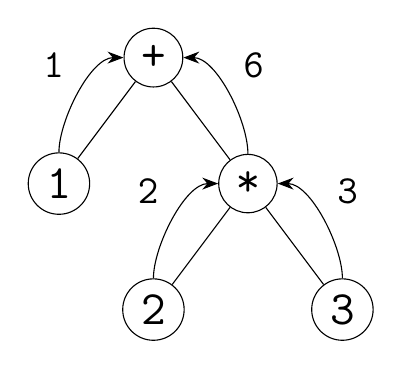
\begin{tikzpicture}[
    arrowtip/.style={
      -{Stealth[scale=1.2]}
    },
    circled/.style={circle,draw,inner sep=3pt},
    leftcurved/.style={
      in control={+(-180:8mm)},
      out control={+(90:8mm)}
    },
    rightcurved/.style={
      in control={+(0:8mm)},
      out control={+(90:8mm)}
    },
    level distance=16mm,
    sibling distance=24mm
  ]
    \node[circled] (Root) at (0,0) {\texttt{+}}
      child {node[circled] (ChildA) {\texttt{1}}}
      child {node[circled] (ChildB) {\texttt{*}}
        child {node[circled] (ChildBA) {\texttt{2}}}
        child {node[circled] (ChildBB) {\texttt{3}}}
      };

    \draw[leftcurved,arrowtip] (ChildA) to (Root);
    \path (ChildA) -- (Root) node[midway,above left=3.5mm] {\small\texttt{1}};

    \draw[rightcurved,arrowtip] (ChildB) to (Root);
    \path (ChildB) -- (Root) node[midway,above right=3.5mm] {\small\texttt{6}};

    \draw[leftcurved,arrowtip] (ChildBA) to (ChildB);
    \path (ChildBA) -- (ChildB) node[midway,above left=3.5mm] {\small\texttt{2}};

    \draw[rightcurved,arrowtip] (ChildBB) to (ChildB);
    \path (ChildBB) -- (ChildB) node[midway,above right=3.5mm] {\small\texttt{3}};
  \end{tikzpicture}
\end{document}
